\documentclass[12pt, a4paper]{article}

\usepackage{amsmath}
\usepackage{amsfonts}
\usepackage{amssymb}
\usepackage{graphicx}
\usepackage{float}
\usepackage{listings}
\usepackage{rotating}
\usepackage{tikz}
\usepackage{verbatim}
\pdfgentounicode=1
\pdfmapline{+cyberb@Unicode@  <cyberbit.ttf}

\begin{document}

\title{BCurve}
\author{P. Baillehache}
\date{\today}
\maketitle

\tableofcontents

\section*{Introduction}

BCurve is C library to manipulate Bezier curves of any dimension and order.\\ 

\section{Interface}

\begin{scriptsize}
\begin{ttfamily}
\verbatiminput{../bcurve.h}
\end{ttfamily}
\end{scriptsize}

\section{Code}

\begin{scriptsize}
\begin{ttfamily}
\verbatiminput{../bcurve.c}
\end{ttfamily}
\end{scriptsize}

\section{Makefile}

\begin{scriptsize}
\begin{ttfamily}
\verbatiminput{../Makefile}
\end{ttfamily}
\end{scriptsize}

\section{Usage}

\begin{scriptsize}
\begin{ttfamily}
\verbatiminput{../main.c}
\end{ttfamily}
\end{scriptsize}

Output:\\
\begin{scriptsize}
\begin{ttfamily}
\verbatiminput{../output.txt}
\end{ttfamily}
\end{scriptsize}

\begin{center}
\begin{figure}[H]
\centering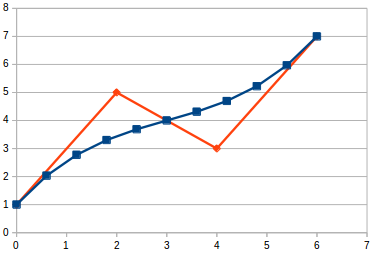
\includegraphics[width=6cm]{./res.png}\\
\end{figure}
\end{center}
\begin{center}
\begin{figure}[H]
\centering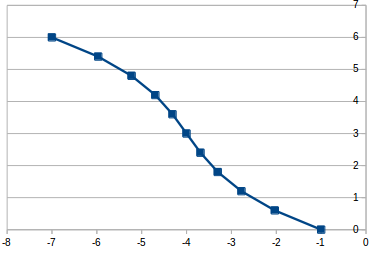
\includegraphics[width=6cm]{./resrot.png}\\
\end{figure}
\end{center}

curve.txt:\\
\begin{scriptsize}
\begin{ttfamily}
\verbatiminput{../curve.txt}
\end{ttfamily}
\end{scriptsize}

\end{document}


